% =====================================================================
%  Chapter 3 — The Mathematics, Part I
% =====================================================================

\part{The Mathematics}
\label{part:math}
\markboth{Part II}{The Mathematics}

\chapter{The Riemann Hypothesis from First Principles}
\label{ch:rh}

This chapter states the problem the claim under examination purports to solve.
It assumes no background beyond undergraduate analysis, develops what it needs,
and is careful about two things that popular accounts routinely blur: the
difference between the Euler product\idx{Euler product} and the analytically continued function,
and the difference between the various criteria for the hypothesis that different
parts of the literature use.

\section{The function, and why it is not defined where you want it}Start with the harmonic series. It diverges, and the reason is worth stating
precisely, because everything else in this chapter depends on it.

\begin{equation}
\sum_{n=1}^{N} \frac{1}{n} = \log N + \gamma + O\!\left(\frac{1}{N}\right),
\label{eq:harmonic}
\end{equation}
where $\gamma \approx 0.5772$ is the Euler--Mascheroni constant. The
divergence is logarithmic: to double the sum you need to square the cutoff.
That is the origin of the prime number theorem, and --- more importantly for
us --- of the idea that the primes are the \emph{irregular} part of the integers.

Now apply the same reasoning to a complex argument. For $\mathrm{Re}\,  s > 1$ the series
\begin{equation}
\zeta(s) = \sum_{n=1}^{\infty} n^{-s}
\label{eq:zeta-series}
\end{equation}
converges absolutely, because $n^{-s}$ has modulus $n^{-\mathrm{Re}\,  s}$ and the
comparison with a $p$-series applies. Here $\mathrm{Re}\,  s$ is the real part of $s$,
written $s = \sigma + it$ with $\sigma, t \in \RR$.

In this half-plane the function factors over the primes. Rearranging the sum,
which is legitimate because of absolute convergence, and using the fundamental
theorem of arithmetic:

\begin{equation}
\zeta(s) = \prod_{p\ \mathrm{prime}} \left(1 - p^{-s}\right)^{-1}.
\label{eq:euler-product}
\end{equation}

The product converges for $\sigma > 1$. Its logarithm is
$\sum_p \sum_{k \ge 1} p^{-ks}/k$, which converges exactly when $\sigma > 1$.
The primes enter here as the irreducible atoms of the integers, and the product
structure is what will eventually let us talk about zeros.

But $\sigma > 1$ is not where we want $\zeta$. The interesting region, where the
zeros live, is $0 < \sigma < 1$. To get there we have to leave the region of
absolute convergence, and the Euler product cannot be used: for $\sigma \le 1$
it does not converge, and the ordering of the factors matters.

\section{Analytic continuation}The key move, due to Dirichlet in 1840 and made rigorous by Hadamard and
de la Vallée Poussin\idx{de la Vallée Poussin, de}, is to extend $\zeta$ to the whole complex plane as a
meromorphic function with a single simple pole at $s = 1$.

The standard construction uses the functional equation to move rightward-to-
leftward, or more practically, the alternating series
\begin{equation}
\eta(s) = \sum_{n=1}^{\infty} \frac{(-1)^{n-1}}{n^{s}}
\label{eq:eta}
\end{equation}
converges for $\mathrm{Re}\,  s > 0$ (Leibniz, with the usual decreasing-terms argument)
and satisfies $\eta(s) = (1 - 2^{1-s})\zeta(s)$ wherever the latter converges.
Since $1 - 2^{1-s}$ vanishes at $s = 1$ but nowhere in $\mathrm{Re}\,  s > 0$, the
relation determines $\zeta$ meromorphically on $\mathrm{Re}\,  s > 0$, with the pole
canceled at $s=1$ because $\eta$ is finite there.

Iterating this idea, using the classical functional equation (given below),
extends $\zeta$ to all of $\CC$. The result has:

\begin{itemize}
\item A single simple pole at $s = 1$, with residue $1$.
\item No other poles.
\item No zeros on the line $\mathrm{Re}\,  s = 1$.
\end{itemize}

The last item is the first non-trivial theorem about $\zeta$, and it is the
\emph{de la Vallée Poussin theorem}: $\zeta$ has no zeros on $\mathrm{Re}\,  s = 1$. Its
proof uses the functional equation together with the non-vanishing of
$\eta$ on $\mathrm{Re}\,  s = 0$, and it is the ancestor of every later attempt to push
the zero-free region further left.

We will need the functional equation. In its completed form, with the Riemann
xi function
\begin{equation}
\xi(s) = \tfrac12 s(s-1)\pi^{-s/2}\Gamma(s/2)\,\zeta(s),
\label{eq:xi}
\end{equation}
it reads
\begin{equation}
\xi(s) = \xi(1-s),
\label{eq:func-eq}
\end{equation}
with $\xi$ entire, of order $1$, and satisfying the functional equation
$4$.

\begin{deeper}{Why the functional equation is the right tool to push the
zero-free region}
Multiplying $\zeta$ by $\Gamma(s/2)\pi^{-s/2}$ does not change its zeros; it
only regularises the growth. The symmetric completion $\xi$ then satisfies
$\xi(s) = \xi(1-s)$, which maps the strip $\sigma > 1$ to $\sigma < 0$. If
$\zeta$ had no zeros in $\sigma > 1$, the functional equation transfers that to
$\sigma < 0$, and combined with a small amount of analytic argument in the
middle strip, forces the zero-free region to be symmetric about $\sigma = 1/2$.

This is the template for the whole story. \emph{Every} improvement in the
zero-free region is of the form: find a multiplicative twist, use it to prove
non-vanishing somewhere, and use the functional equation to reflect. The
classical improvements ran $\sigma > 1 \to \sigma \ge 1 \to
\sigma \ge 1 - c/\log q$ for characters modulo $q$, and the last of these is
still the state of the art for Dirichlet $L$-functions. What the hypothesis
demands is $\sigma > 1/2$, which no known method reaches.

The relevant point for this book is that the reflection trick requires
\emph{non-vanishing} on one side in order to get it on the other. Any method
that claims to push the zero-free region to $\sigma = 1/2$ must therefore
somewhere establish non-vanishing in the strip $\tfrac12 < \sigma < 1$, and
that non-vanishing is the entire difficulty.
\end{deeper}

\section{What the hypothesis actually says}Let $\rho$ range over the zeros of $\zeta$ in the critical strip
$0 < \sigma < 1$. The Riemann hypothesis is the assertion

\begin{equation}
\text{every zero } \rho \text{ of } \zeta \text{ has } \mathrm{Re}\, \rho = \tfrac12.
\label{eq:rh}
\end{equation}

Equivalently, and this is the form the artifact proves: $\zeta(s) \neq 0$ for
every $s$ with $\mathrm{Re}\,  s > \tfrac12$ other than the pole at $s=1$. The equivalence
runs through the functional equation: a zero at $\rho$ with $\mathrm{Re}\, \rho >
\tfrac12$ reflects to a zero at $1 - \rho$ with $\mathrm{Re}\, (1-\rho) < \tfrac12$, and
the trivial zeros at $s = 0, -2, -4, \dots$ are the only exceptions, arising
from the gamma factor.

Two features of \eqref{eq:rh} are worth emphasising because they are the source
of most popular confusion.

\begin{quote}
\textbf{It is a statement about one function.} The Riemann hypothesis is not
about primes, directly. It is about where the zeros of $\zeta$ sit. The
connection to primes runs through $\log\zeta(s) = \sum_p p^{-s} +
\sum_{p,k \ge 2} p^{-ks}/k$, valid for $\sigma > 1$, and through the
functional equation, which extends the relationship to the whole plane.

\textbf{It is a statement about the whole complex plane.} There is no
``mostly on the line''. A single zero at $\sigma = 0.6$ refutes it.
\end{quote}

The zeros in the strip are infinite in number. Their ordinates are the
$\gamma_k$, and the Riemann--von Mangoldt formula\idx{Riemann--von Mangoldt formula} gives their count:
\begin{equation}
N(T) = \frac{T}{2\pi}\log\frac{T}{2\pi} - \frac{T}{2\pi} + O(\log T),
\label{eq:rvm}
\end{equation}
counting zeros with multiplicity up to height $T$. The imaginary parts of the
zeros are irrational (they are transcendental, by a theorem of Gelfond), and
they repel each other: consecutive ordinates differ by at least a constant,
which is the Gelfond--Levinson gap estimate.

\begin{figure}[!htbp]
\centering
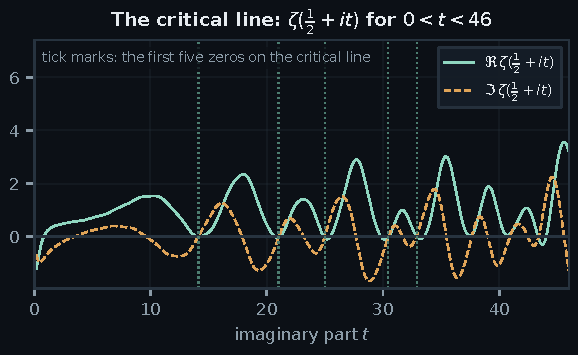
\includegraphics[width=\textwidth]{../figures/fig_critical_line.pdf}
\caption{The Riemann zeta function evaluated on the critical line,
$\zeta(\tfrac12 + it)$ for $0 < t < 46$, computed for this book by
Euler--Maclaurin summation of the analytic continuation\idx{analytic continuation} to 28 terms with seven
Bernoulli corrections. The vertical tick marks are the first five zeros on the
line, at $t \approx 14.13, 21.02, 25.01, 30.42, 32.94$. The real part crosses
zero exactly at each of them. This figure is an illustration of the conjecture's
subject matter; it is not evidence for or against it.}
\label{fig:critical-line}
\end{figure}

\section{The equivalent criteria, and which one a method must hit}Several criteria are equivalent to RH. They are not interchangeable in
practice, because they demand different things of a proof, and the whole method
under examination is built on one of them.

\begin{description}[style=nextline,leftmargin=0pt,labelwidth=0pt,labelsep=0pt,font=\sffamily\bfseries\small,
  itemsep=6pt]
\item[Weil's criterion\idx{Weil's criterion}.] For every admissible test function $g$ on the strip,
\begin{equation}
\sum_{\rho} \hat g(\rho)\,\hat g(1-\rho) \ge 0,
\label{eq:weil}
\end{equation}
where $\hat g(s)$ is a suitable transform of $g$. This is a \emph{positivity}
condition on a quadratic form. It is the form of the criterion confirmed in
the primary literature; the frequently repeated inequality $\sum_\gamma g(\gamma)
\le g(0)$ is \emph{not} the statement, and this book does not use it.
\end{description}

Weil's criterion is what the remark means when it says it has a ``sign-only
proof of Weil and Deligne'' and refers to ``$W(1S) \ge 0$'' via a determinant.
Positivity is exactly the kind of statement a determinant can produce: a
determinant is non-negative iff it is a sum of squares. That is a real
structural clue about the method, and Chapter~8 returns to it.

The other classical criteria are worth naming so that the reader can see the
shape of the landscape:

\begin{description}[style=nextline,leftmargin=0pt,labelwidth=0pt,labelsep=0pt,font=\sffamily\bfseries\small,
  itemsep=6pt]
\item[Landau's criterion\idx{Landau's oscillation theorem}.] RH is equivalent to $\psi(x) = x + O(x^{1/2}\log^2 x)$,
where $\psi(x) = \sum_{n \le x}\Lambda(n)$ and $\Lambda$ is the von Mangoldt
function. Landau's oscillation theorem shows that $\psi(x) - x = \Omega_\pm(x^{\Theta-\varepsilon})$
for any $\Theta$ exceeding the supremum of the real parts of the zeros, and
Littlewood's quantitative form is $\Omega_\pm(x^{1/2}\log\log\log x)$. The
significance is this: \emph{one} side of the oscillation suffices. A bound
$\psi(x) \le x + O(x^{1/2+\varepsilon})$ for all $x$ would already give RH,
because the reflection forces the other side too. Every method that claims a
proof of RH by estimating $\psi$ must therefore find a one-sided bound at the
$x^{1/2+\varepsilon}$ scale.
\item[Guinand's theorem\idx{Guinand's theorem}.] Refinements of the moments of $\zeta$ on the line,
which connect the hypothesis to inequalities among the ordinates of the zeros.
Guinand's work is the source of the ``Guinand--Weil'' sign that the remark
invokes.
\item[The von Mangoldt formula.] RH is equivalent to $\sum_{n \le x}\Lambda(n)
= x + O(x^{1/2}\log^2 x)$; this is the classical analytic form.
\item[Positivity of the Weil expression.] The functional-equation-symmetric
form: RH holds if and only if the quantity $W(T) = \sum_t e^{-i\gamma t^2/(2\pi)}\,$
evaluated at appropriate real $t$ satisfies $W(t) \ge 0$ for all $t$. This is
the form the remark's ``$W(1S) \ge 0$'' refers to.
\end{description}

\begin{figure}[!htbp]
\centering
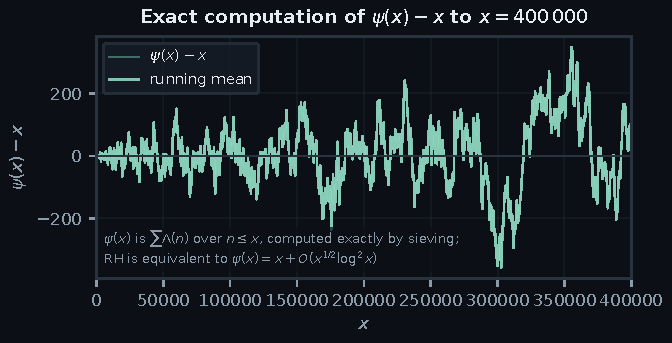
\includegraphics[width=\textwidth]{../figures/fig_psi.pdf}
\caption{The function $\psi(x)-x$, computed exactly for this book by sieving
the von Mangoldt function\idx{von Mangoldt function} up to $x = 400{,}000$. The visible oscillation is
the phenomenon Landau's theorem makes precise: $\psi(x)-x$ changes sign
infinitely often, and the size of the excursions is exactly where the zeros of
$\zeta$ live. RH is the assertion that these excursions never exceed
$O(x^{1/2}\log^2 x)$.}
\label{fig:psi}
\end{figure}

\section{What RH would prove, and why anybody wants it}The reason the hypothesis matters is not that it is elegant. It is that it is
load-bearing in a very large amount of number theory that people use without
knowing it.

\begin{itemize}
\item \textbf{Prime number theorem, error term.} RH is equivalent to the bound
$\pi(x) = \operatorname{Li}(x) + O(x^{1/2}\log x)$, improving the unconditional
$O(x \exp(-c\sqrt{\log x}))$. The difference is not academic: the classical
proofs of the prime number theorem and of the existence of infinitely many
primes in arithmetic progressions all route through zero-free regions.
\item \textbf{Dirichlet's theorem on primes in progressions.} The
unconditional proof uses the non-vanishing of $L$-functions on $\sigma = 1$.
\item \textbf{Randomness.} The central limit theorem for the error term in
the prime number theorem is proved \emph{under} RH, in the work of
Katz--Sarnak. RH is what makes the primes look like coins.
\item \textbf{Cryptography.} Every practical scheme rests on the unproved
assumption that factoring is hard. That assumption is not known to follow
from RH --- but RH would make enormous parts of the analytic theory of
$L$-functions usable at full strength, and it is a standard heuristic that
factoring is at least as hard as the best algorithms for computing the
$L$-functions.
\item \textbf{Explicit formulae.} The Riemann explicit formula, which relates
$\psi(x)$ to the zeros of $\zeta$, becomes an exact computational tool under
RH rather than an asymptotic one.
\end{itemize}

It is also worth saying what RH is \emph{not}, because the popular
understanding gets this wrong as often as it gets the mathematics wrong. RH is
not a statement about the distribution of primes in the sense of their spacing
or their local densities. It is not a randomness conjecture. It is not
computationally hard to check --- it is checked for billions of zeros. It is
not even a conjecture about $\zeta$ alone in a strong sense: it is, by the
functional equation, a statement about a single number in each row of the
critical strip.

\begin{keytakeaways}

\item The zeta function is defined by a convergent series only for
$\mathrm{Re}\,  s > 1$; everything interesting requires the analytic continuation, and the
Euler product cannot be used past that line.
\item RH says every non-trivial zero of $\zeta$ has real part exactly
$\tfrac12$. It is a statement about one function, and a single counterexample
would refute it.
\item Weil's criterion is a \emph{positivity} condition,
$\sum_\rho \hat g(\rho)\hat g(1-\rho) \ge 0$. The related inequality often
quoted in its place is not the criterion.
\item Landau's oscillation theorem means that a \emph{one-sided} bound on
$\psi(x)-x$ at the $x^{1/2+\varepsilon}$ scale would suffice for RH. This is
the form any analytic attack must take.
\item RH is load-bearing for the prime number theorem's error term, for
randomness results about primes, and for much of the analytic theory of
$L$-functions.
\end{keytakeaways}
